\documentclass[11pt]{article}

\usepackage{amsmath,amssymb,algorithmic,algorithm,graphicx}
\usepackage[margin=1in]{geometry}


\title{Machine Learning\\ Assignment 3}
\author{Daniel Leblanc}
\date{March 20, 2013}

\begin{document}
\maketitle

\paragraph{Experiment 1:} The ROC curve was created using a Python script.  The code is included in the file 'rocCurve.py' and is attached.  The points on the curve are determined by the number of entries in each threshold rather than being divided on the values in the prediction file.  From the ROC curve you can tell that the trained SVM is more likely to classify a non-spam e-mail as spam than it is to classify a spam e-mail as non-spam.  The curve is quite smooth and the true positive rate is higher than the false positive positive rate in the optimal position at the top left of the graph.
\begin{center}
  Accuracy: 89.62\%
\end{center}

\begin{center}
  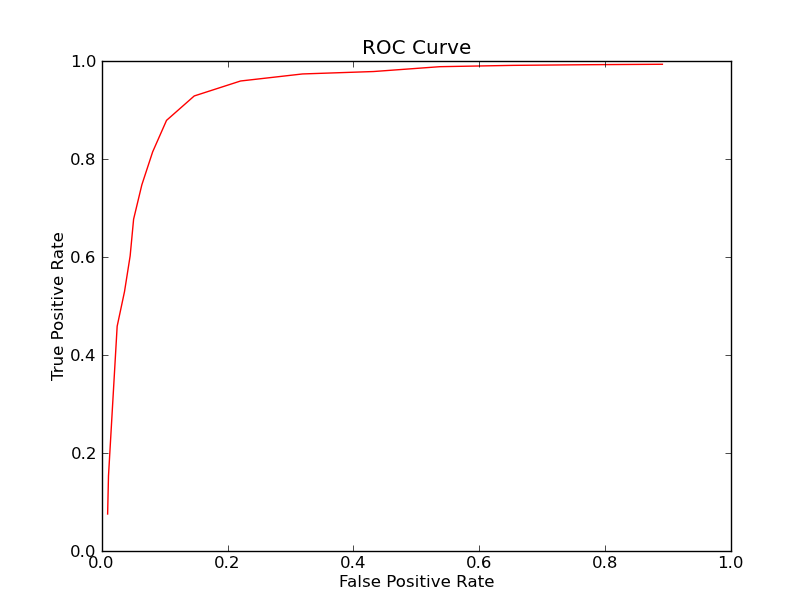
\includegraphics[width=6.0in]{q1curve.png}
\end{center}

\paragraph{Experiment 2:} The Adaboost algorithm was also implemented in Python and the code is included in the file adaboost.py.  When run the code automatically executes svm learn and svm classify as required to create the 10 models and their associated alpha values that are needed to apply the algorithm to the test data.  The code will then run the test data through each of the 10 models that were created and generate a new spam.predictions file that rocCurve.py can be run against to generate the ROC curve seen below.  I was quite surprised to find that the boosted results were less accurate than the results from the first experiment.  I spent a couple days trying to find a problem in my code that would explain why the boosted results were consistently worse than those of the original model, without success.  My code seems to exactly perform the Adaboost algorithm as it is defined on the slides from lecture.  There may be something that I've missed, but I have been unable to find any explanation or issue with my program.  As for the ROC curve the conclusions I can draw are basically the same as the results from experiment 1.  I'm not really sure why the ROC curve is more jagged than the previous results.
\begin{center}
  Accuracy: 87.42\%
\end{center}

\begin{center}
  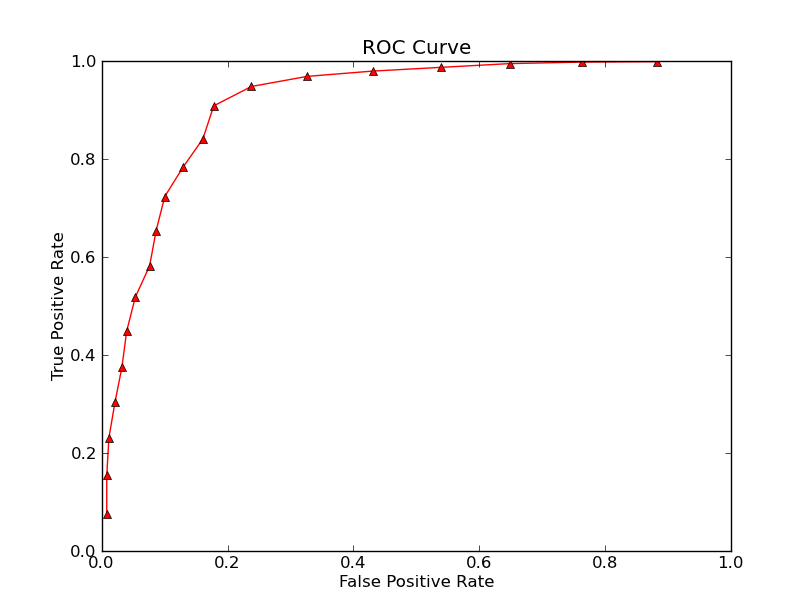
\includegraphics[width=6.0in]{q2curve.png}
\end{center}

\paragraph{Experiment 3:} The difference between the results from this run and the previous test is barely noticable.  The tiny improvement in accuracy was not consistent over multiple runs.  Any conclusions I could draw from this result are really no different than the ones from the previous two experiments.
\begin{center}
  Accuracy: 87.80\%
\end{center}

\begin{center}
  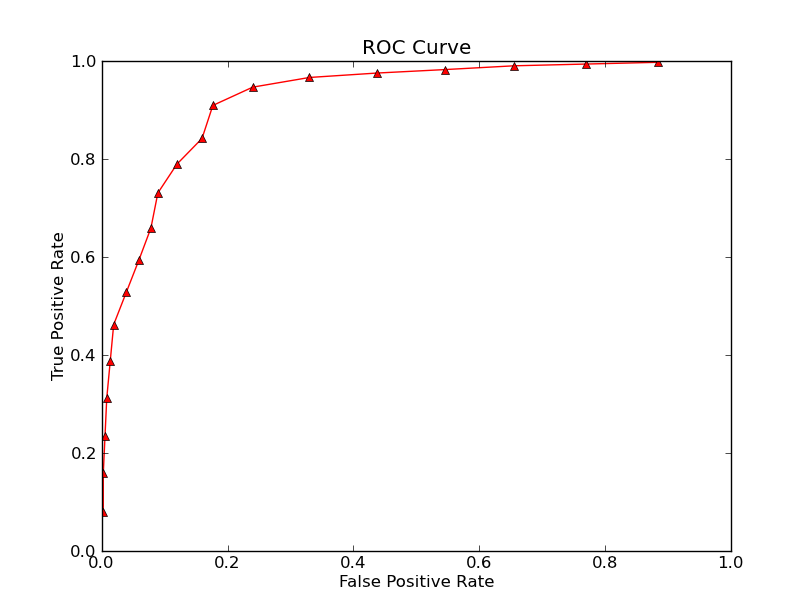
\includegraphics[width=6.0in]{q3curve.png}
\end{center}

\paragraph{Conclusion:} The SVM method itself is impressively effective for such a simple way of classifying data.  The boosting I'm still pretty lost on.  Based on my understanding of the method, the likelyhood of it getting worse results should be quite low, but that is what happened for me.  I'm still convinced that there must be something wrong with the code I implemented, but have been totally unable to figure out what.  I'll probably try to tackle this task a second time, but it will have to wait for me to finish a few of my other projects.  I'll try to build a simpler system and avoid some of the automated system calls to make it easier to debug.  The Adaboost algorithm is clearly based on sound principles and I found it very frustrating not being able to get useful results.

\end{document}